\documentclass{beamer}
\usetheme{Warsaw}

\usepackage[utf8]{inputenc}
\usepackage{fancybox}
\usepackage{multimedia} 
\usepackage{subfig}
\usepackage{amsmath}
\usepackage{hyperref}
\usepackage[all]{xy}
\begin{document}


\title[Angewandte Mathematik] % (optional, only for long titles)
{Angewandte Mathematik
\\
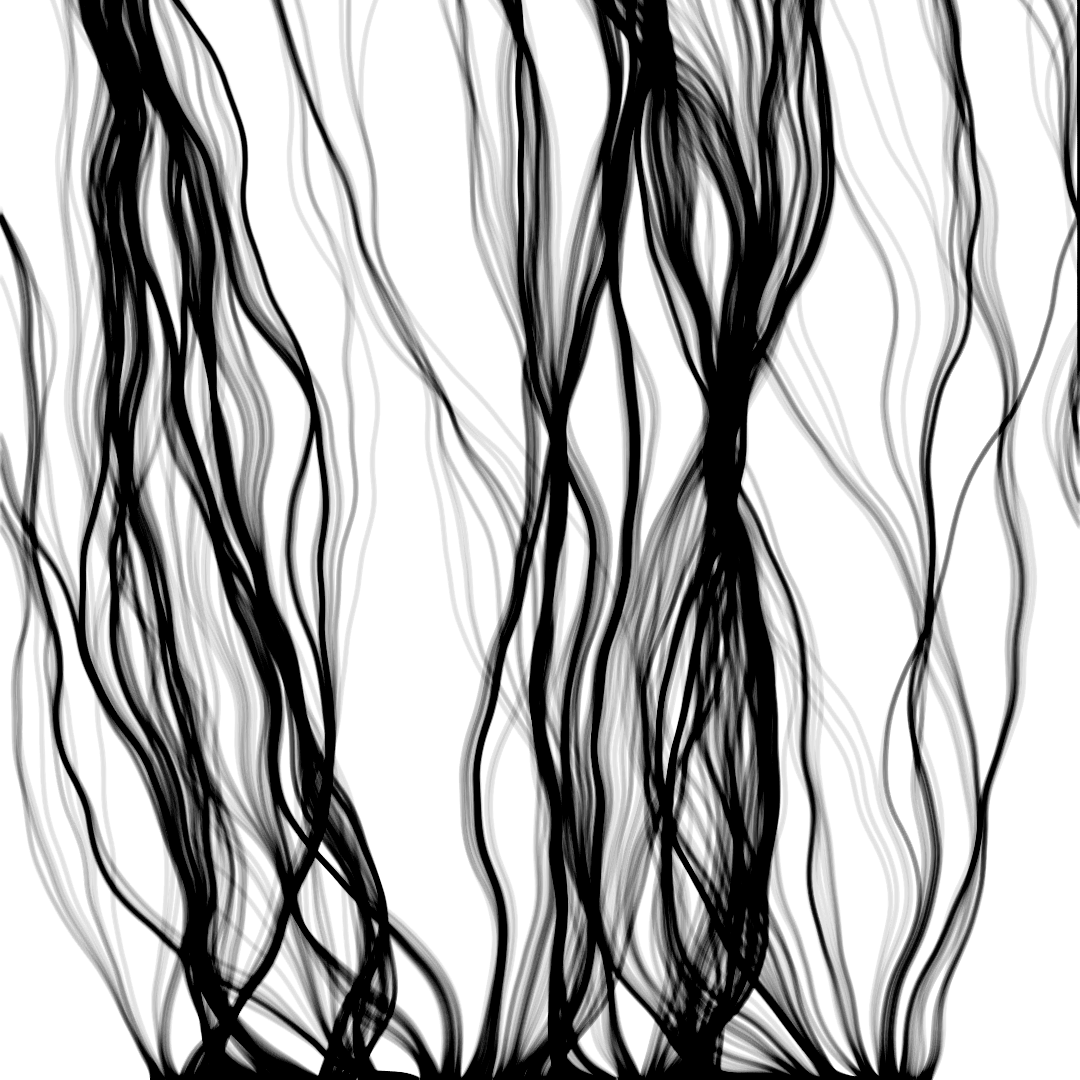
\includegraphics[scale=0.15]{images/cover}
}
\subtitle{}
\author[Dr. Johannes Riesterer] % (optional, for multiple authors)
{Dr.  rer. nat. Johannes Riesterer}

\date[KPT 2004] % (optional)
{}

\subject{Angewandte Mathematik}




\begin{frame}
    \frametitle{Angewandte Mathematik}
\framesubtitle{Gradientenverfahren}
    \begin{block}{Gradientenverfahren}
Wie kann man Minima einer  differenzierbaren Abbildung $f: \mathbb{R}^n \to \mathbb{R}$ finden? 
 
\end{block}

    \begin{block}{Gradientenverfahren}
\begin{itemize}
\item An jedem Punkt $x_k \in  \mathbb{R}^n$ zeigt der negative Gradient  $d_k := -\nabla f (x_k)$ in die steilste Abstiegsrichtung.
\item Für hinreichend kleines $\alpha_k$ folgt mit Satz über die lokale Linearisierung:
$f(x_{k+1}) = f (x_k + \alpha_k d_k) =  f(x_k) + \alpha_k df(x_k)d_k + R( \alpha_k dk)$
\item  Setze $x_{k+1} = x_k + \alpha_k d_k$ 
\item Es gilt $f(x_{k+1}) \leq f(x_k)$, falls $\nabla f(x_k) \neq 0$
\item  Falls die folge $f(x_k)$ beschränkt ist, so ist  dieser Fixpunkt $x^*$ ein Minimum, da $\nabla f(x^*) = 0$ gelten muss.  
\end{itemize}

\end{block}
 \end{frame}



\begin{frame}
    \frametitle{Angewandte Mathematik}
\framesubtitle{Gradientenverfahren}
\begin{figure}[H]
      \centering
    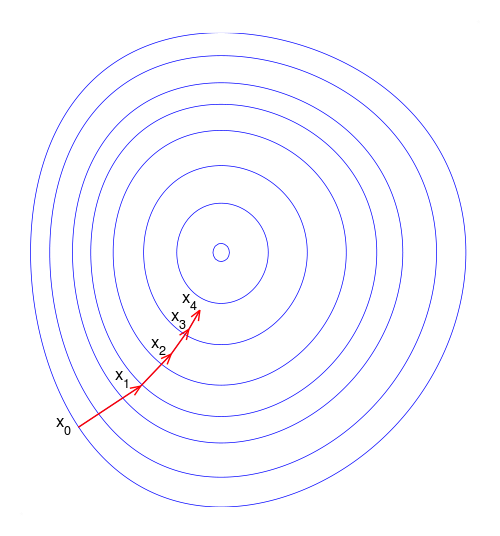
\includegraphics[width=0.5\textwidth]{images/Gradient_descent}
      \caption{Quelle: Wikipedia}
\end{figure}

 \end{frame}




\begin{frame}
    \frametitle{Angewandte Mathematik}
\framesubtitle{Gradientenverfahren}
    \begin{block}{Höhenlinien}
Sei  $f: \mathbb{R}^n \to \mathbb{R}$  eine differenzierbare Funktion. Eine Kurve $\gamma : I \to \mathbb{R}^n$, auf der $f$ konstant ist, also 
$f(\gamma(t)) = c$ für ein festes $c \in \mathbb{R}$ gilt, heißt Höhenlinie.
\end{block}

\begin{figure}[H]
      \centering
    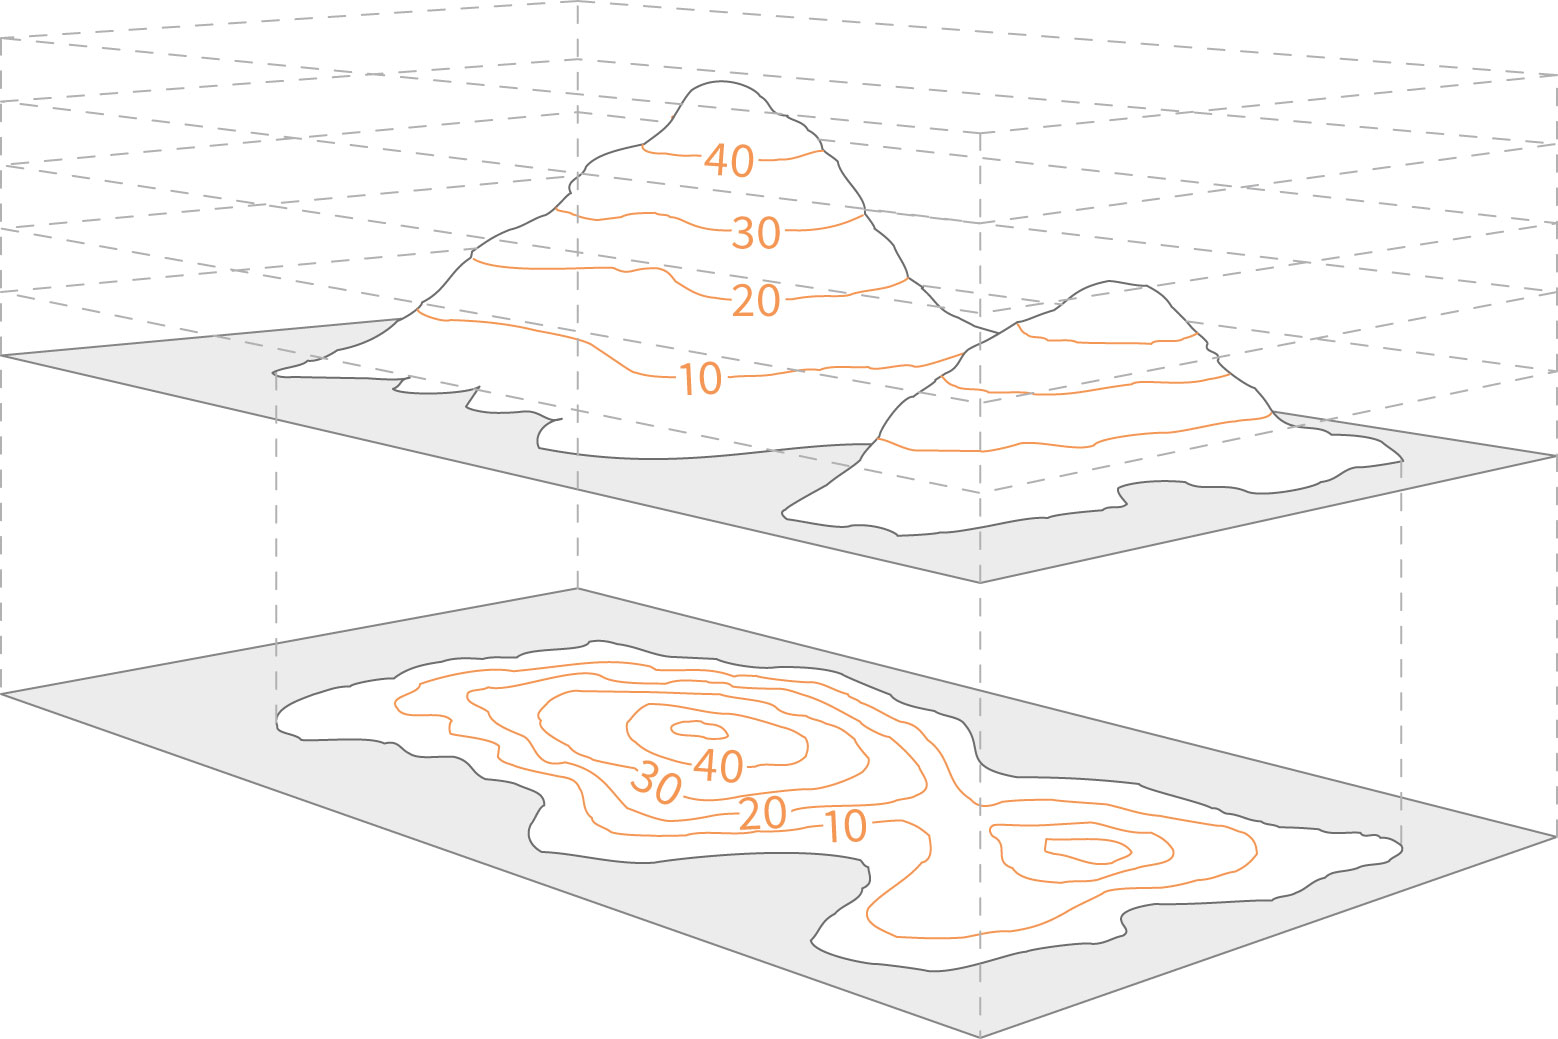
\includegraphics[width=0.5\textwidth]{images/Contours-and-relief}
      \caption{Quelle: https://getoutside.ordnancesurvey.co.uk/guides/understanding-map-contour-lines-for-beginners/}
\end{figure}

 \end{frame}


\begin{frame}
    \frametitle{Angewandte Mathematik}
\framesubtitle{Gradientenverfahren}
    \begin{block}{Höhenlinien}
Der Gradient steht senkrecht auf  Höhenlinien. Dies bedeutet, dass $$ \bigl \langle \nabla f(\gamma(t)), \gamma'(t) \bigr \rangle = 0$$ gilt. 

\end{block}
    \begin{block}{Beweis}
Aus $f(\gamma(t)) = c$ folgt $\frac{d}{dt} f(\gamma(t)) = 0$. Mit der Kettenregel folgt $\frac{d}{dt} f(\gamma(t)) =  df(\gamma(t)) \cdot \gamma'(t) = 0$ und damit
$ \bigl \langle \nabla f(\gamma(t)), \gamma'(t) \bigr \rangle = 0$.
\end{block}

 \end{frame}



\begin{frame}
    \frametitle{Angewandte Mathematik}
\framesubtitle{Backpropagation}
    \begin{block}{Backpropagation}
Das Gradientenverfahren angewendet auf eine Lossfunktion eines neuronalen Netzes wird als Backpropagation bezeichnet.
Gegeben ist ein neuronales Netz $f : \Omega \times \mathbb{R}^n \to \mathbb{R}^m$, 
und ein  Datensatz $D : = \{ (x_i, y_i) \}$ mit $x_i \in \mathbb{R}^n, y_i \in \mathbb{R}^m$. Finde Gewichte Omega, so dass Lossfunktion
\begin{align*}
L_D  : \Omega \subset \mathbb{R}^n \to \mathbb{R} 
\end{align*}
minimal wird. Zum Beispiel $$L_D(\omega) := \sum_{(x_i,y_i) \in D} (f(\omega, x_i) - y_i)^2$$.

\end{block}
 \end{frame}


\begin{frame}
    \frametitle{Angewandte Mathematik}
\framesubtitle{Backpropagation}
 \begin{figure}[!tbp]
  \centering
  \begin{minipage}[b]{0.45\textwidth}
    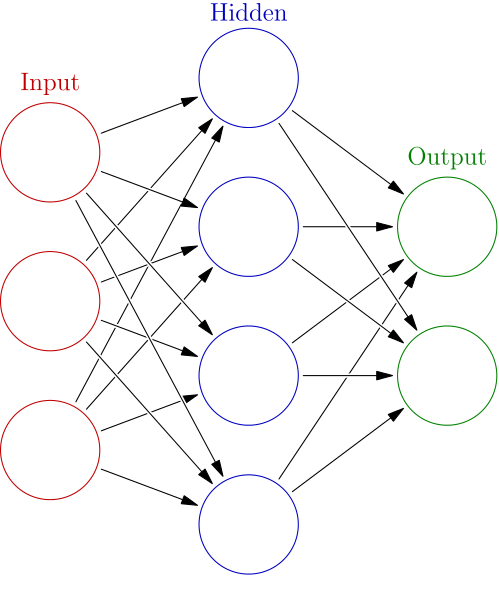
\includegraphics[width=0.6\textwidth]{images/499px-Colored_neural_network}
    \caption{}
  \end{minipage}
  \hfill
  \begin{minipage}[b]{0.45\textwidth}
    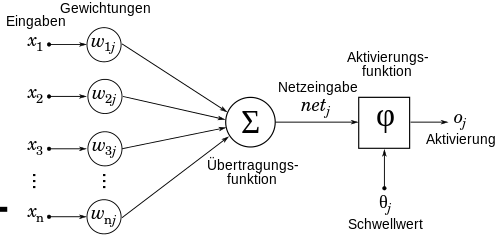
\includegraphics[width=1.0\textwidth]{images/500px-NeuronModel_deutsch}
    \caption{}
  \end{minipage}
\end{figure}
 \end{frame}


\begin{frame}
    \frametitle{Angewandte Mathematik}
\framesubtitle{Backpropagation}
    \begin{block}{Backpropagation}
\begin{itemize}
\item  Initialisiere $k:=0$ und zufällige Gewichte $w_0$.
\item \pause Initialisiere Genauigkeit $\epsilon > 0$
\item \pause   \text{While } {$|| \nabla L_D(\omega) || > \epsilon$}  
\item \pause Bestimme $\alpha_k$  mit $ L_D(\omega_k + \alpha d_k) =  L_D(\omega_k) + \alpha_k d L_D(\omega_k)d_k + R( \alpha_k dk)$ 
\item \pause  Setze $\omega_{k+1} := \omega_k  + \alpha_k d_k$. 
\item \pause $k \leftarrow k+1$
\end{itemize}
\end{block}
 \end{frame}

\begin{frame}
    \frametitle{Angewandte Mathematik}
\framesubtitle{Backpropagation}
    \begin{block}{Mini Batch}
\begin{itemize}
\item   Datensatz $D$ sehr groß (Big Data)
\item \pause Berechnung des Gradienten der Lossfunktion entsprechend aufwendig. 
\item \pause Wende Backpropagation auf Teilräume $D' \subset D$ an (Minibatch).
\item \pause $\#D' = 1$ stochastischer Gradientenabstieg.
\end{itemize}

\end{block}
 \end{frame}



\begin{frame}
    \frametitle{Angewandte Mathematik}
\framesubtitle{Minibatch}
\begin{figure}[H]
      \centering
    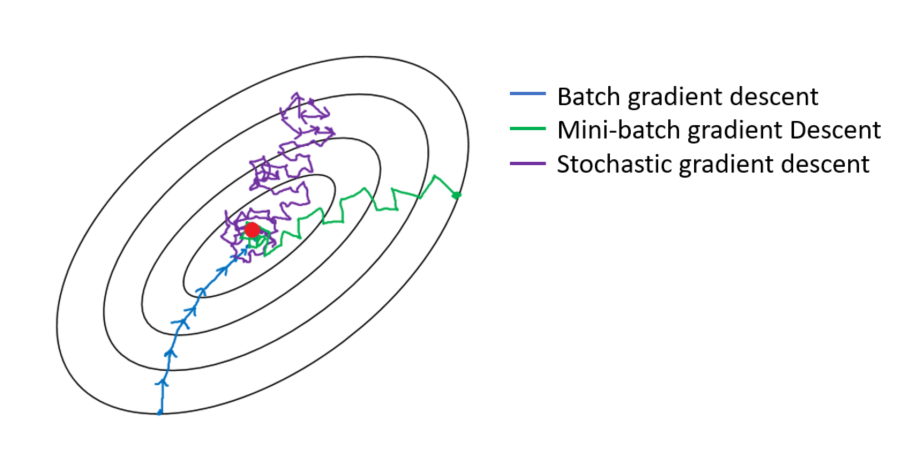
\includegraphics[width=1.0\textwidth]{images/batchgradient}
      \caption{Quelle: https://towardsdatascience.com/batch-mini-batch-stochastic-gradient-descent-7a62ecba642a}
\end{figure}

 \end{frame}



\begin{frame}
    \frametitle{Angewandte Mathematik}
\framesubtitle{Backpropagation}
    \begin{block}{Backpropagation}
\begin{itemize}
\item  Initialisiere $k:=0$ und zufällige Gewichte $w_0$.
\item \pause Initialisiere Genauigkeit $\epsilon > 0$
\item \pause Wähle Teilmenge $D_0' \subset D$
\item \pause   \text{While } {$|| \nabla L_{D_k'}(\omega) || > \epsilon$}  
\item \pause Bestimme $\alpha_k$  mit $ L_{D_k'}(\omega_k + \alpha d_k) =  L_{D_k'}(\omega_k) + \alpha_k d L_{D_k'}(\omega_k)d_k + R( \alpha_k dk)$ 
\item \pause  Setze $\omega_{k+1} := \omega_k  + \alpha_k d_k$. 
\item \pause Wähle neue Teilmenge $D'_{k +1} \subset D$.
\item \pause $k \leftarrow k+1$
\end{itemize}
\end{block}
 \end{frame}


\begin{frame}
    \frametitle{Angewandte Mathematik}
\framesubtitle{Automatisches Ableiten}
\begin{figure}[H]
      \centering
    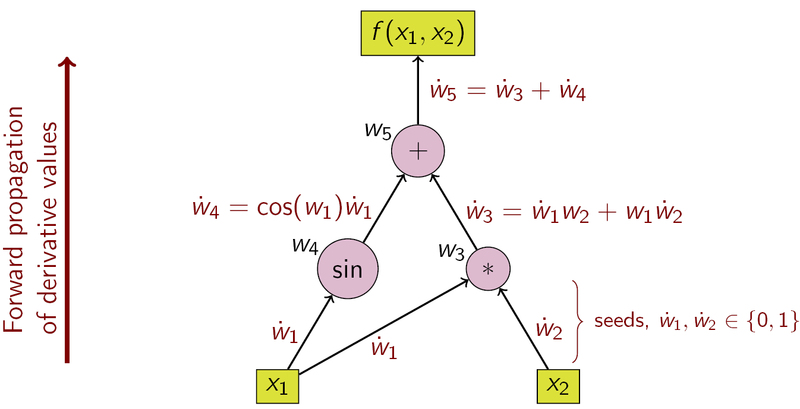
\includegraphics[width=0.8\textwidth]{images/ad.png}
      \caption{Quelle: Wikipedia}
\end{figure}

\href{https://pytorch.org/tutorials/beginner/blitz/autograd_tutorial.html}{Automatisches Ableiten  in Pytorch}

\href{https://jax.readthedocs.io/en/latest/notebooks/quickstart.html}{Automatisches Ableiten  in JAX}

 \end{frame}



\begin{frame}
    \frametitle{Angewandte Mathematik}
\framesubtitle{Backpropagation}
    \begin{block}{Konditionszahl}
Ist $f : U \to \mathbb{R}^m$ differnzierbar, so lässt dich mit dem Mittelwertsatz die Konditionszahlen berechnen durch
\begin{align*}
& \kappa = || f'(x) || \\
& \kappa_{rel} = \frac{||x||}{|| f(x)||} ||f'(x) ||
\end{align*}
mit der Operatornorm 
$||h|| : = \sup_{||x|| =  1} ||h(x)||$

\end{block}
 \end{frame}

\begin{frame}
    \frametitle{Angewandte Mathematik}
\framesubtitle{Backpropagation}
    \begin{block}{Konditionszahl Addition/Subtraction}
Für $f:(x,y):= x \pm y$ ist $f'(x,y) = (1,\pm 1)$ und dem Betrag als Norm auf $\mathbb{R}$  und der Norm $||(x,y)|| := |x| + |y|$ ist 
\begin{align*}
& \kappa = 1 \\
& \kappa_{rel} = \frac{|a| + |b| }{|a \pm b|}
\end{align*}
Für die Addition ist  $\kappa_{rel} = 1$ und damit gut konditioniert.
Für die Subtraktion zweier fast gleich großer Zahlen ist $|a - b| << |a| + |b|$ und damit ist in diesem Fall $\kappa_{rel} >> 1$ und damit schlecht konditioniert. 
\end{block}
 \end{frame}



\end{document}

